\section{Matchings}
\label{sec:matchings}

\newcommand{\maxcardmatch}{\hyperref[prob:max_matching]{\textsf{Maximum Cardinality Matching}}}
\newcommand{\symdiff}{\ensuremath{\bigtriangleup}}
\newcommand{\odd}[1]{\ensuremath{\f[\mathrm{odd}]{#1}}}
%\subsection{Introduction and Notation}

\begin{definition}[Matching]
    Given a graph $G = (V, E)$, a matching $M \sse E$ is a set of edges such that no two edges in $M$ share 
    a common vertex. 
    \label{def:matching}
    \begin{definition}[Covered/Exposed]
        A node is $M$-covered if some edge in $M$ is incident to it. Else it is $M$-exposed. 
    \end{definition}
\end{definition}

Note that a matching $M$ covers exactly $2\abs{M}$ nodes, leaving $\abs{V} - 2\abs{M}$ nodes exposed. 
A matching is \emph{maximal} if adding any edge $e \in E \sm M$ to it causes it to no longer be a matching. 
A matching is \emph{perfect} if it covers all the nodes. A basic decision problem is to decide if a graph has a perfect matching. 
The following theorem gives a way to determine if a graph has a perfect matching. 

\begin{theorem}[Tutte's Matching Theorem]
    A graph $G =\lrp{V, E}$ has a perfect matching iff for every subset $A$ of nodes, $\odd{G \sm A} \leq \abs{A}$, 
    where $\odd{\cdot}$ denotes the number of connected components having an odd number of nodes.  
    \label{thm:tutte_matching}
\end{theorem}

A more general problem is to find a maximum cardinality matching. 

\begin{problem}[Maximum Cardinality Matching]
    Given a graph $G = (V, E)$, find a matching $M$ that has maximum cardinality. Equivalently, find a 
    matching with the fewest exposed nodes. 
    \label{prob:max_matching}
\end{problem}

\subsection{Augmenting Paths}

A path $P$ is a collection of edges $\lrp{v_0, v_1}, \ldots, \lrp{v_{k-1}, v_k} = e_1, \ldots, e_k $ where each $v_i$ is distinct.   

\begin{definition}[Alternating Path]
    Given a matching $M$ in a graph $G$, a path $P$ in $G$ is $M$-alternating if it alternates
    between edges in $M$ and edges in $E \sm M$. 
    \label{def:alternate_path}
\end{definition}

\begin{definition}[Augmenting Path]
    Given a matching $M$ in a graph $G$, a path $P$ in $G$ is $M$-augmenting if it is $M$-alternating and  
    its end nodes are distinct and $M$-exposed. 
    \label{def:augment_path}
\end{definition}

We use the notation $A \symdiff B = \lrp{A \cup  B} \sm \lrp{A \cap B}$ to denote the symmetric difference of $A$ and $B$
(i.e.\! the set of elements unique to $A$ and $B$).
\begin{lemma}
    If $M$ is a matching and $P$ an $M$-augmenting path, then $M^\prime = M \symdiff P$ is a matching that 
    contains one more edge than $M$. 
    \label{lem:augment_path_matching}
\end{lemma}
\begin{proof}
    By definition of an $M$-augmenting path, $P$ is of odd length with edges in $M$ occurring at every even index. 
    Therefore, $M^\prime = M \symdiff P$ contains the edges of $M \sm P$ and edges of $P$ at odd indices, which covers all nodes covered by $M$ plus the end nodes of $P$ 
    and contains exactly one more edge than $M$. 
\end{proof}

Augmenting paths can be used to identify a \maxcardmatch{} in the following way. 

\begin{theorem}[Augmenting Path Theorem]
    A matching $M$ in a graph $G$ is maximum iff there is no $M$-augmenting path. 
    \label{thm:augmenting_path}
\end{theorem}
\begin{proof}
    $\Longrightarrow$ (by contrapositive): Direct consequence of \cref{lem:augment_path_matching}. 
\end{proof}
\begin{proof}
    $\Longleftarrow$ (by contrapositive): Let $M^{\ast}$ be a maximum matching. Let $Q = M^{\ast} \symdiff M$. 
    Then each node is incident to at most one edge in $M^{\ast} \cap Q$ and one edge in $M \cap Q$. Hence, $Q$ is an edge set 
    of node disjoint paths and circuits where edges alternate between belonging in $M^{\ast}$ and $M$. 
    Because the edges are taken from matchings, all circuits must be of even length 
    and contain the same number of edges from $M^{\ast}$ and $M$. Therefore, since $\abs{M^{\ast}} > \abs{M}$, 
    there must be at least one path in $Q$ that contains more edges from $M^{\ast}$ than $M$. Such a path is 
    $M$-augmenting. 
\end{proof}

\subsection{Alternating Trees}

Let $M$ be a current matching and $X$ the set of $M$-exposed nodes. 

\begin{definition}[Alternating Tree]
    An $M$-alternating tree is a tree $T$ with root node $r \in X$ such that along every path to a node $v$, 
    the path is $M$-alternating with $e_i \in M$ iff $i = 2k$ for some $k \in \Z^+$. 
    \label{def:alternating_tree}
\end{definition}

\begin{figure}[h]
    \centering
    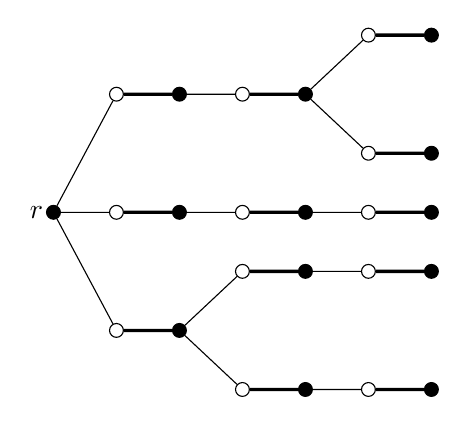
\begin{tikzpicture}
        [
            level distance=8mm,
            every node/.style={draw, fill, circle, minimum size=5pt, inner sep=0pt, line width=0.4pt},
            rootnode/.style={label=left:$r$},
            level 1/.style={nodes={fill=none}, edge from parent/.append style={line width=0.4pt}},
            level 2/.style={nodes={fill}, edge from parent/.append style={line width=1.2pt}},
            level 3/.style={nodes={fill=none}, edge from parent/.append style={line width=0.4pt}},
            level 4/.style={nodes={fill}, edge from parent/.append style={line width=1.2pt}},
            level 5/.style={nodes={fill=none}, edge from parent/.append style={line width=0.4pt}},
            level 6/.style={nodes={fill}, edge from parent/.append style={line width=1.2pt}},
            edge from parent/.style={draw}
        ]

        \node[rootnode] (root) at (0,0) {} [grow = east]
            child {node {} 
                child {node {}
                    child {node {}
                        child {node {} 
                            child {node {}
                                child {node {} 
                                }
                            }
                        }
                    }
                    child {node {}
                        child {node {} 
                            child {node {}
                                child {node {} 
                                }
                            }
                        }
                    }
                }
            } 
            child {node {} 
                child {node {}
                    child {node {} 
                        child {node {}
                            child {node {} 
                                child {node {}}
                            }
                        }
                    }
                }
            }
            child {node {} 
                child {node {}
                    child {node {} 
                        child {node {}
                            child {node {} 
                                child {node {}} 
                            }
                            child {node {} 
                                child {node {}} 
                            }
                        }    
                    }
                }
            };
    \end{tikzpicture}
    \caption{An example of an alternating tree. Nodes in $A_T$ are white while nodes in $B_T$ are black.}
    \label{fig:alternating_tree}
\end{figure}

We can divide an alternating tree $T = (V_T, E_T)$ into two node sets $A_T$ and $B_T$ such that $A_T$ is the set of nodes 
at the other end of an odd-length $M$-alternating path starting at $r$ and $B_T$ is the set of nodes at the other end 
of an even-length $M$-alternating path starting at $r$. Such sets can be built by the following relation: 
starting with $A_T = \emptyset$ and $B_T = \lrc{r}$, if $\lrp{u, v} \in E$ such that $u \in B_T$ and $v \notin A_T \cup B_T$ and there 
exists an edge $\lrp{v, w} \in M$, then $A_T \gets A_T \cup \lrc{v}$ and $B_T \gets B_T \cup \lrc{w}$. 
Note that $\abs{B_T} = \abs{A_T} + 1$. 
Additionally, if there exists some 
edge $\lrp{i, j}$ where $i \in B_T$ and $j \notin T$ such that $j$ is $M$-exposed, then the path $P = \lrp{r, v_1}, \ldots, \lrp{i, j}$
is $M$-augmenting. 

\begin{definition}
    An $M$-alternating tree is \emph{maximal} if for all $b \in B_T$, $\f[N]{b} \sse V_T$ (i.e.\! no additional nodes can be added to the tree).
    It is \emph{frustrated} if for all $b \in B_T$, $\f[N]{b} \sse A_T$.
    \label{def:maximal_alternating_tree}
\end{definition} 

Alternating trees are useful in deciding if a graph has a perfect matching in the following way. 

\begin{lemma}
    Suppose that $G$ has a matching $M$ and an $M$-alternating tree $T$ that is frustrated. Then $G$ has no perfect matching. 
    \label{lem:frustrated_tree_perfect_matching}
\end{lemma}
\begin{proof}
    Consider $G \sm A_T$. The nodes $B_T$ are then single node odd components of $G \sm A_T$ by definition of
    a frustrated tree. Therefore, 
    \begin{equation*}
        \odd{G \sm A_T} \geq \abs{B_T} > \abs{A_T}
    \end{equation*}
    which fails the condition of \cref{thm:tutte_matching}. 
\end{proof}

\subsection{Maximum Cardinality Matchings in the Bipartite Case}

\begin{algorithm}[!h]
    \caption{Maximum Cardinality Matching in Bipartite Graphs} \label{alg:max_card_match_bipartite}
    \begin{algorithmic}[1]
        \Algin A bipartite graph $G = \lrp{V, E}$
        \Algout A matching $M$ 
        \State $X \gets V, M \gets \emptyset, \calT \gets \emptyset$ \Comment{$X$ is the set of $M$-exposed nodes}
        \While{$X \neq \lrc{\f[\mathrm{root}]{T_i} \colon T_i \in \calT}$} \label{line:max_card_bi_while}
            \State $T \gets \Call{MaximalTree}{G}$%\Call{MaximalTree}{G, X \cap V, M \cap E}$
            \State $\calT \gets \calT \cup T$%, $X \gets X^\prime$, $M \gets M \cup M^\prime$
            \State $G \gets G \sm T$ \Comment{Remove subgraph $T$ from $G$}
        \EndWhile
        \State \Return $M$
        \Statex
        \Function{MaximalTree}{$G = \lrp{V, E}$}
            \State Choose $r \in X \cap V$ \Comment{Choose $M$-exposed vertex in current graph}
            \State $T \gets \lrp{\lrp{A, B}, E_T}$ where $A = \emptyset$, $B = \lrc{r}, E_T = \emptyset$  
            \While{$\exists e = \lrp{u, v} \in E$ where $u \in B$, $v \notin T$}
                \If{$v \in X$} \Comment{Forms an $M$-augmenting path}
                    \State Let $P$ be the path from $r$ to $v$
                    \State $M \gets \Call{Augment}{M, P}$
                    \State $X \gets X \sm \lrc{r, v}$ 
                    \If{$X = \emptyset$}
                        \State \Return $\emptyset$ %$\lrp{\emptyset, \emptyset, M}$ 
                        \Comment{$M$ is a perfect matching}
                    \Else 
                        \State Choose $r \in X \cap V$ \Comment{Start a new $M$-alternating tree}
                        \State $T \gets \lrp{\lrp{\emptyset, \lrc{r}}, \emptyset}$ 
                    \EndIf
                \Else
                    \State $T \gets \Call{ExtendTree}{T, e}$
                \EndIf
            \EndWhile
            \State \Return $T$ %$\lrp{T, X, M}$ 
            \Comment{A maximal $M$-alternating tree is returned}
        \EndFunction
        \Statex
        \Procedure{Augment}{$M$, $P$}
            \State \Return $ M \symdiff P$
        \EndProcedure
        \Statex
        \Procedure{ExtendTree}{$T = \lrp{\lrp{A, B}, E_T} , e = \lrp{u, v}$}
            \If{$\exists e^\prime = \lrp{v, w} \in M$}
                \State $A \gets A \cup \lrc{v}$
                \State $B \gets B \cup \lrc{w}$    
                \State $E_T \gets E_T \cup \lrc{e, e^\prime}$
            \EndIf
        \EndProcedure
    \end{algorithmic}  
\end{algorithm}

We first note the following. 
\begin{lemma}
    Let $G$ be a bipartite graph. Consider a tree $T$ returned by $\Call{MaximalTree}{G}$. $T$ is maximal. 
    \label{lem:bi_max_card_match_maximal_tree_frustrated}
\end{lemma}
\begin{proof}
    It suffices to show that there exists no edge between any two nodes $b_1, b_2 \in B$. By construction of $T$, if such 
    an edge were to exist, it would form an odd length cycle as any two nodes in $B$ always have an even length path in $T$. 
    However, since $G$ is bipartite, it is impossible for it to have an odd length cycle. Therefore, for all $b \in B$, $\f[N]{b} \sse A$, 
    and $T$ is maximal and frustrated. 
\end{proof}

As an immediate consequence of \cref{lem:frustrated_tree_perfect_matching} and \cref{lem:bi_max_card_match_maximal_tree_frustrated}, 
we get the following. 

\begin{corollary}
    If in the first iteration of \cref{alg:max_card_match_bipartite} a tree $T$ is returned by $\Call{MaximalTree}{G}$, 
    then $G$ has no perfect matching. 
    \label{cor:maximal_tree_bi_no_perf}
\end{corollary}

The correctness of \cref{alg:max_card_match_bipartite} is based on the following. 

\begin{theorem}
    Let $G$ be a graph, $M$ a matching on $G$, and $X$ the set of $M$-exposed nodes. Let $\calT$ be a maximal forest of (disjoint) maximal $M$-alternating trees.  
    Define $A = \bigcup_{T_i \in \calT} A_{T_i}$ and $B = \bigcup_{T_i \in \calT} B_{T_i}$. If 
    \begin{itemize}[label=--]
        \item $X = \lrc{\f[\mathrm{root}]{T_i} \colon T_i \in \calT}$
        \item There are no edges between nodes in $B$ 
    \end{itemize}
    then $M$ is a maximum cardinality matching. 
    \label{thm:general_maximal_m_alt_trees_maximum_card}
\end{theorem}
\begin{proof}
    By assumption, there are no edges between nodes in $B$. 
    %Additionally, there are no edges between nodes in $B$ and nodes not in $A \cup B$ as they would have been marked as being in $A$ when creating the $M$-alternating trees. 
    Therefore, all edges with an endpoint in $B$ must have the other endpoint in $A$. 

    By definition of an $M$-alternating tree $T_i$, we have that $\abs{B_{T_i}} - \abs{A_{T_i}} = 1$ with the root node being $M$-exposed. Thus, across all trees we have that 
    $\abs{B} - \abs{A} = \abs{\calT}$ (i.e.\! there are $\abs{T}$ $M$-exposed nodes). 
    For a matching to be of greater cardinality than $M$, it must have fewer than $\abs{\calT}$ exposed nodes. 
    However, such a matching still needs to match each node of $B$ onto a node of $A$, so it is not possible for it to have fewer exposed nodes. 
    Therefore, $M$ is a maximum cardinality matching. 
\end{proof}

As the above theorem applies to general graphs, we get the following for bipartite graphs.  

\begin{theorem}
    If $G$ is bipartite, the matching $M$ that \cref{alg:max_card_match_bipartite} returns is a maximum cardinality matching. 
    \label{thm:bipartite_max_card_matching}
\end{theorem}
\begin{proof}
    As shown in \cref{lem:bi_max_card_match_maximal_tree_frustrated}, the algorithm must 
    return a forest $\calT$ of maximal $M$-alternating trees such that for each tree $T_i$, there exists no edge between nodes in $B_{T_i}$. 
    Additionally, there do not exist any edges between nodes of $B_{T_i}$ and $B_{T_j}$ for $i \neq j$ as when the first of the two trees 
    were being constructed, such an edge would have been used to extend the tree. 
    Moreover, by design of the algorithm, it must be that $X = \lrc{\f[\mathrm{root}]{T_i} \colon T_i \in \calT}$. 
    Therefore, by \cref{thm:general_maximal_m_alt_trees_maximum_card} $M$ is a maximum cardinality matching. 
\end{proof}

\subsection{Minimum Weight Perfect Matchings in the Bipartite Case}

If edges are given weights, we can look at the question of finding a perfect matching of minimum 
weight.

\begin{problem}[Minimum Weight Perfect Matching]
    Given a graph $G = (V, E)$ that can have a perfect matching and an edge weight function $w\colon E \to \R$, find a perfect matching $M$ of 
    minimum weight. 
    \label{prob:min_weight_perf_match}
\end{problem}

This can be formulated as an IP as shown below where the $x_e$ are binary variables denoting 
whether an edge is in the matching or not. 

\begin{mini}
    {}{\sum_{e \in E} w_e x_e}{}{\label{lp:min_weight_perf_match_ip}}{}
    \addConstraint{\sum_{e \in E\colon v \in e} x_e}{= 1}{\quad \forall v \in V}
    \addConstraint{x_e}{\in \lrc{0, 1}}{\quad \forall e \in E}
\end{mini}

To facilitate this in a bipartite graph $G = (V = (A, B), E)$, %we can add edges with infinite weight if they do not exist to make the bipartite graph complete. 
we can reformulate \cref{lp:min_weight_perf_match_ip} 
to emphasize the properties of the bipartite graph. We now have binary variables $x_{ij}$ where $i \in A$ and $j \in B$
to denote whether the edge $\lrp{i, j}$ is in the matching or not. 
\begin{mini}
    {}{\sum_{i \in A, j \in B} w_{ij} x_{ij}}{}{\label{lp:min_weight_perf_match_ip_bipartite}}{}
    \addConstraint{\sum_{j \in B} x_{ij}}{= 1}{\quad \forall i \in A}
    \addConstraint{\sum_{i \in A} x_{ij}}{= 1}{\quad \forall j \in B}
    \addConstraint{x_{ij}}{\in \lrc{0, 1}}{\quad \forall i \in A, j \in B}
\end{mini}
The LP relaxation of this IP is given by letting $x_{ij} \geq 0$. 
\begin{mini}
    {}{\sum_{i \in A, j \in B} w_{ij} x_{ij}}{}{\label{lp:min_weight_perf_match_lp_bipartite}}{}
    \addConstraint{\sum_{j \in B} x_{ij}}{= 1}{\quad \forall i \in A}
    \addConstraint{\sum_{i \in A} x_{ij}}{= 1}{\quad \forall j \in B}
    \addConstraint{x_{ij}}{\geq 0}{\quad \forall i \in A, j \in B}
\end{mini}
The dual is given by 
\begin{maxi}
    {}{\sum_{i \in A} u_i + \sum_{j\in B} v_j }{}{\label{lp:min_weight_perf_match_dual_lp_bipartite}}{}
    \addConstraint{u_i + v_j}{\leq w_{ij}}{\quad \forall i \in A, j \in B}
\end{maxi}
where $u_i$ denotes nodes in the $A$ partition and $v_j$ nodes in the $B$ partition. 

A theorem by Birkhoff shows that the optimal value of \cref{lp:min_weight_perf_match_lp_bipartite} is equivalent to the 
optimal value of \cref{lp:min_weight_perf_match_ip_bipartite}. Therefore, by \cref{thm:strong_duality} we have that an optimal 
feasible solution to the dual \cref{lp:min_weight_perf_match_dual_lp_bipartite} gives an optimal feasible solution to \cref{lp:min_weight_perf_match_ip_bipartite}.  

\begin{theorem}[Birkhoff]
    Let $G$ be a bipartite graph with edge weight function $w\colon E \to \R$. Then $G$ has a perfect matching iff 
    \cref{lp:min_weight_perf_match_lp_bipartite} has a feasible solution. Moreover, if $G$ has a perfect matching, then the minimum weight 
    of a perfect matching is equal to the optimal value of \cref{lp:min_weight_perf_match_lp_bipartite}.  
    \label{thm:birkhoff}
\end{theorem}

Define $\overline{w}_{ij} = w_{ij} - \lrp{u_i + v_j}$. A solution to \cref{lp:min_weight_perf_match_dual_lp_bipartite} is feasible iff $w_{ij} \geq 0$ for all $i \in A, j \in B$. 
By \cref{cor:complementary_slack} we have that a complementary slackness condition for optimal solutions to \cref{lp:min_weight_perf_match_lp_bipartite} and \cref{lp:min_weight_perf_match_dual_lp_bipartite} is 
\begin{equation}
    x_{ij} > 0 \Longleftrightarrow \overline{w}_{ij} = 0. 
    \label{eq:min_weight_perf_match_slac}
\end{equation}
If $\lrp{u, v}$ are solutions to \cref{lp:min_weight_perf_match_dual_lp_bipartite}, denote by $\f[E_=]{u, v}$ 
the set $\lrc{\lrp{i, j} \in E \colon \overline{w}_{ij} = 0}$. By the complementary slackness condition, this implies that if $M$ is an optimal perfect matching described by vector $x$, 
then $M \sse  \f[E_=]{u, v}$ for an optimal dual solution $\lrp{u, v}$. However, for a given dual solution $\lrp{u, v}$, we may not be able to find a perfect matching among the edges of $\f[E_=]{u, v}$. 

Given some feasible dual solution $\lrp{u, v}$, we can use the $\Call{MaximalTree}{}$ function in \cref{alg:max_card_match_bipartite} to 
search for a perfect matching in $G_= = \lrp{V, E_=}$. 
%If the algorithm returns no tree, it returns a perfect matching of $G_=$, whose characteristic vector $x$
%is a feasible solution of \cref{lp:min_weight_perf_match_lp_bipartite} and satisfies the complementary slackness conditions with the current dual solution, so it must be optimal. 
Otherwise, the algorithm returns a matching $M$ of $G_=$ and an $M$-alternating tree $T$ such that 
nodes of $B_T$ are joined to nodes in $A_T$ by edges of $E_=$. 

In this case, we want to update the dual solution in such a way that its value increases. 
By definition of an $M$-alternating tree $T$ in a bipartite graph, we know that $A_T$ and $B_T$ belong to separate partitions. WLOG assume that $A_T \sse A$ and $B_T \sse B$. 
We can update the dual by keeping the edges of of $M$ and $T$ in $\f[E_=]{u, v}$ and decreasing the $\overline{w}_{cd}$ for edges $(c, d)$ such that $c \in B_T$ and $d \notin A_T$. 
The decrease can be achieved by choosing some $\varepsilon = \min \lrc{\overline{w}_{cd} \colon c \in B_T, d \notin T}$
and decreasing $u_i$ by $\varepsilon$ for all $i \in A_T$ and increasing $v_j$ by $\varepsilon$ for all $j \in B_T$. 
The dual is clearly still feasible as $\overline{w}_{ij} \geq 0$ for $i \in A, j \in B$ and some edge
joining a node $c \in B_T$ and $d \notin T$ will enter $E_=$. Since this new node $d \notin T$, it can lead to either an augmentation or 
tree extension step. We can iteratively continue doing this until a perfect matching is returned 
or stop when we get a frustrated tree. 

\begin{algorithm}[!h]
    \caption{Minimum Weight Perfect Matching in Bipartite Graphs} \label{alg:min_weight_perf_match_bi}  
    \begin{algorithmic}[1]
        \Algin A bipartite graph $G = (V, E)$, a feasible dual solution $\lrp{u, v}$, a matching $M$ of $G_=$
        \Algout Either a perfect matching $M$ or a NO certificate
        \State Let $X$ be the set of $M$-exposed nodes. Choose $r \in X$
        \State $T \gets \lrp{\lrp{A, B}, E_T}$ where $A = \emptyset, B = \lrc{r}, E_T = \emptyset$  
        \While{$T$ is not frustrated}
            \While{$\exists e = \lrp{c, d} \in E_=$ where $c \in B, d \notin T$}
                \If{$d \in X$}      
                    \State Let $P$ be the path from $r$ to $d$  
                    \State $M \gets \Call{Augment}{M, P}$
                    \State $X \gets X \sm \lrc{r, d}$
                    \If{$X = \emptyset$}
                        \State \Return $M$ \Comment{$M$ is a perfect matching}
                    \Else 
                        \State Choose $r \in X$
                        \State $T \gets \lrp{\lrp{\emptyset, \lrc{r}}, \emptyset}$ 
                    \EndIf 
                \Else 
                    \State $T \gets \Call{ExtendTree}{T, e}$
                \EndIf
            \EndWhile
            \State $\varepsilon \gets \min \lrc{\overline{w}_{cd} \colon c \in B_T, d \notin T}$
            \State $u_i \gets u_i - \varepsilon$ for all $i \in A$, $v_j \gets v_j + \varepsilon$ for all $j \in B$
        \EndWhile
        \State \Return NO \Comment{No perfect matching exists}
        \Statex
        \Procedure{Augment}{$M$, $P$}
            \State \Return $ M \symdiff P$
        \EndProcedure
        \Statex
        \Procedure{ExtendTree}{$T = \lrp{\lrp{A, B}, E_T} , e = \lrp{u, v}$}
            \If{$\exists e^\prime = \lrp{v, w} \in M$}
                \State $A \gets A \cup \lrc{v}$
                \State $B \gets B \cup \lrc{w}$    
                \State $E_T \gets E_T \cup \lrc{e, e^\prime}$
            \EndIf
        \EndProcedure
    \end{algorithmic}
\end{algorithm}

The correctness of this algorithm is based on the fact that if a perfect matching is returned,
we get a corresponding characteristic vector $x$ and a feasible dual solution $\lrp{u, v}$ that satisfy 
the complementary slackness condition \cref{eq:min_weight_perf_match_slac}. By \cref{cor:complementary_slack}, they must 
therefore be optimal solutions to \cref{lp:min_weight_perf_match_lp_bipartite} and \cref{lp:min_weight_perf_match_dual_lp_bipartite}, respectively. 
By \cref{thm:birkhoff}, this gives that the matching $M$ returned is of minimum weight. 

\begin{theorem}
    \cref{alg:min_weight_perf_match_bi} can be implemented in $\bigO{n^2m}$ time where 
    $n = \abs{V}, m = \abs{E}$. 
    \label{thm:min_weight_perf_match_bi_runtime}
\end{theorem}
\begin{proof}
    In the worst case, the algorithm may perform only one tree extension in an iteration of the outer while loop, 
    and thus requires a dual change during this iteration. This gives $\bigO{n^2}$ dual changes. 
    A naive way to compute $\varepsilon$ for each dual change is to just look at every edge, so in total we get 
    a running time of $\bigO{n^2m}$. 
\end{proof}
